\chapter{Présentation de l'entreprise}
\chaptermark{Présentation Générale}
\minitoc
\newpage
 
\section{Présentation de l'Entreprise ECONOCOM}
Econocom est une entreprise française spécialisée dans la conception, le financement
et l’accompagnement de la transformation digitale des systèmes d’information de ses clients.
Soutenue par plus de 9 000 collaborateurs répartis dans 19 pays, et un chiffre d’affaires qui
dépasse les 3 milliards d’euros pour l’année 2018, Econocom dispose de plusieurs moyens
technologiques et financiers ainsi qu’un niveau élevé d’expertise pour la réussite des grands
projets digitaux, services aux infrastructures, conseil applicatifs et solutions métiers.
Depuis 2015, Econocom a acquis le statut de Société Européenne. Cotée sur Euronext
à Bruxelles depuis 1986, l’action Econocom Group fait partie des indices Bel Mid et Tech40.

\begin{figure}[h]
\begin{center}
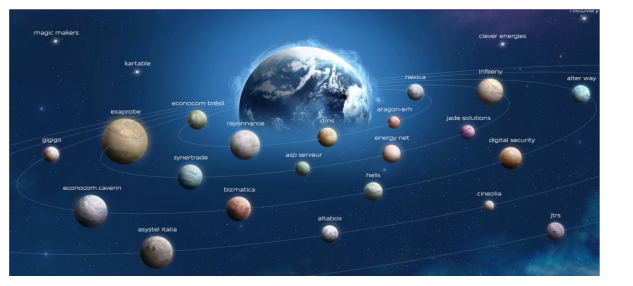
\includegraphics[scale=0.70]{Organigramme_Econocom.png}
\caption[Organigramme du groupe]{Organigramme du groupe}
\label{monlabel}
\end{center}
\end{figure}


Comme le montre le schéma de la Figure1, Econocom présente une organisation
innovante inspirée de la voie lactée, la Galaxie, comme on l’appelle au sein de la société. La planète Econocom comporte toutes les activités historiques, en constante expansion et qui restent entièrement possédées par le groupe. Des petites et moyennes entreprises représentées par des satellites, dans plusieurs domaines principalement rattachés au monde du digital. Les entrepreneurs dirigeants et généralement fondateurs conservent une part significative dans le capital social de l’entreprise, ce qui leurs permet une meilleure maitrise et une totale autonomie. Econocom compte aujourd’hui 19 sociétés, positionnées dans les domaines stratégiques de la sécurité, du développement d’applications web et mobile, des solutions digitales en mode cloud, et du conseil en transformation digitale.

Les tailles de ces sociétés sont en proportion avec leur contribution au chiffre
d’affaires du groupe. On peut citer les plus performantes en terme de chiffre d’affaire :

•   Exaprobe : C’est l’intégrateur du groupe Econocom. Avec plus de 15 années  
d’expérience, son métier est de définir, intégrer et exploiter, chez le client ou dans le Cloud, des infrastructures et solutions Réseaux, Sécurité, Communications Unifiées et Audiovisuelles.

•   Infeeny : Elle offre à ses clients un accompagnement et des solutions Microsoft
adaptées pour répondre aux enjeux de la transformation digitale. Infeeny regroupe plus de 330 collaborateurs et se positionne dans le top 3 des spécialistes Microsoft en France.

%\begin{figure}[h]
%\begin{center}
%\includegraphics[scale=0.70]{performance_industrielle.png}
%\caption[Processus de la performance industrielle]{Processus de la performance industrielle}
%\label{monlabel}
%c
%\end{figure}

%\newpage
%\section{Les chiffres clés}
%\begin{center}
%\includegraphics[scale=0.80]{Chiffre_cles.png}
%\label{monlabel}
%\end{center}
%\newpage

\section{Les domaines d'expertise chez ECONOCOM}
Econocom met en œuvre pour et avec ses clients, du conseil, des projets  d’approvisionnement et de gestion administrative des actifs numériques, des services aux infrastructures, des applicatifs et des solutions métiers et le financement de ces projets.
Nous détaillons ci-dessous, les différents domaines d’expertises, mais aussi les entités (BU) qui les prennent en charge :
\newline
• La Cyber Sécurité est assurée par Digital Security et Exaprobe. Ils font du conseil, de l’audit et de l’expertise en sécurité numérique et notamment celle des IOT (Internet Of Things) ou des objets connectés.
\newline
•  Microsoft est assurée par Infeeny.
\newline
•  Web Apps, SaaS et Cloud : ces services sont assurés par Alter Way, Aragon-ERH, ASP Serveur, Econocom Brésil, Nexica, Synertrade Infrastructure et réseaux : Asystel Italia, ASP Serveur, Exaprobe et Nexica offrent une panoplie de services et solutions comme les services d’hébergement critique On-Demand, réseau et infogérance.
\newline
•  Mobilité : Bizmatica, DMS, Econocom Brésil, GIGIGO, Jade Solutions, JTRS et Rayonnance mettent en œuvre des solutions qui vont accélérer le processus de transformation numérique des entreprises en se focalisant et en mettant en avant l’expérience utilisateur, qui devient essentielles pour l’adoption d’un nouveau produit / services.
\newline
•  Digital Signage et Multimedia : assuré par Altabox, Caverin, Cineolia, Energy Net, cette entité permet la conception et le déploiement de solutions d’affichage dynamique, du marketing sensoriel et d’analyse de trafic de données avec pour objectif l’amélioration de l’expérience client et l’accélération des ventes.
\newline
• Conseil : Helis, spécialiste en conseil stratégique, AMOA et Direction de projet, offrant ainsi à Econocom une brique supplémentaires qui lui permet de mieux répondre aux besoins de ses clients.

\begin{figure}[h]
\begin{center}
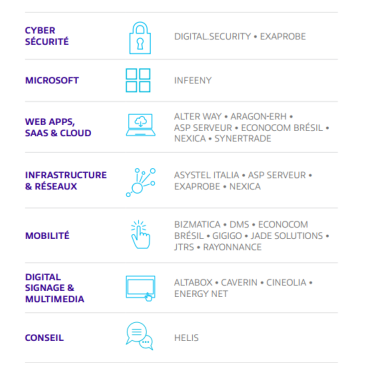
\includegraphics[scale=0.70]{Domaines_Econocom.png}
\caption[Les domaines d'expertise chez ECONOCOM]{Les domaines d'expertise chez ECONOCOM}
\label{monlabel}
\end{center}
\end{figure}






